\section{Esercizio 4 -- Shift Register}
\subsection{Esercizio 4.1}
Implementiamo uno shift register di N bit utilizzando sia un approccio comportamentale, sia un approccio strutturale.

\subsubsection{Implementazione comportamentale}
\begin{code}
    \inputminted{vhdl}{vhdl/shiftregister_behavioral.vhd}
    \caption{Implementazione dello shift register comportamentale}
    \label{cod:shiftregister_behavioral}
\end{code}

Un registro a scorrimento è un circuito sequenziale che memorizza i dati in un array di bit e li sposta a destra o a sinistra in base ai segnali di controllo.

Il [Codice sorgente \ref{cod:shiftregister_behavioral}] è suddiviso in tre parti principali:

\begin{enumerate}
    \item Dichiarazione dell'entità:
    \begin{itemize}
        \item L'entità \texttt{shiftregister\_behavioral} ha un parametro generico \texttt{bit\_number}, che specifica la lunghezza del registro (di default 8 bit).
        \item I segnali di input e output includono il clock (\texttt{clock}), il reset (\texttt{reset}), il segnale di caricamento (\texttt{load}), un segnale di selezione (\texttt{Y}), il controllo del verso dello shift (\texttt{shift\_left}), un vettore di input (\texttt{input}), e un vettore di output (\texttt{output}).
    \end{itemize}
    \item Dichiarazione della variabile interna:
    \begin{itemize}
        \item \texttt{bit\_array}: un vettore di bit che rappresenta il registro a scorrimento.
    \end{itemize}
    \item Processo sequenziale sincronizzato con il clock:
    \begin{itemize}
        \item Se il reset è attivo (\texttt{reset = `1'}), il registro viene azzerato.
        \item Se il load è attivo (\texttt{load = `1'}), il registro viene caricato con il valore di \texttt{input}.
        \item Altrimenti, viene eseguito lo shift:
        \begin{itemize}
            \item Se \texttt{shift\_left = `1'}, lo shift avviene verso sinistra.
            \item Se \texttt{shift\_left = `0'}, lo shift avviene verso destra.
            \item Il segnale \texttt{Y} determina di quanti bit eseguire lo shift:
            \begin{itemize}
                \item Se \texttt{Y = `0'}, il registro si sposta di 1 bit.
                \item Se \texttt{Y = `1'}, il registro si sposta di 2 bit.
            \end{itemize}
        \end{itemize}
    \end{itemize}
\end{enumerate}

\subsubsection{Implementazione strutturale}
\begin{code}
    \inputminted{vhdl}{vhdl/shiftregister_structural.vhd}
    \caption{Implementazione dello shift register strutturale}
    \label{cod:shiftregister_structural}
\end{code}

L'approccio \texttt{structural} [Codice sorgente \ref{cod:shiftregister_structural}] consiste nel suddividere il sistema in componenti più piccoli e collegarli tra loro.

Il registro ha un numero di bit configurabile (\texttt{bit\_number}) e può:
\begin{itemize}
    \item Caricare un valore esterno (\texttt{load}).
    \item Azzerarsi (\texttt{reset}).
    \item Effettuare lo shift dei bit a destra o sinistra.
    \item Shiftare di 1 o 2 posizioni, a seconda del valore del segnale \texttt{Y}.
\end{itemize}

\paragraph{Funzionamento Generale.}
L'implementazione strutturale si basa su tre componenti fondamentali:
\begin{enumerate}
    \item Flip-flop D (\texttt{flipflop\_D}): memorizza il valore di ogni bit ad ogni fronte di clock [Codice sorgente \ref{cod:flipflop_D}].
    \item Multiplexer 2:1 (\texttt{mux\_2\_1}): sceglie se caricare un nuovo valore o continuare con il valore shiftato [Codice sorgente \ref{cod:mux_2_1}].
    \item Multiplexer 4:1 (\texttt{mux\_4\_1}): seleziona da quale posizione deve arrivare il bit durante lo shift [Codice sorgente \ref{cod:mux_4_1}].
\end{enumerate}

\paragraph{Struttura dell'architettura.}
L'architettura [Figura \ref{fig:4_1_SHIFTREGISTER_STRUCTURAL}] è composta da una serie di segnali interni e da una generazione di componenti tramite ciclo \texttt{generate}. I segnali interni sono:

\begin{itemize}
    \item \texttt{bit\_array}: memorizza lo stato attuale del registro.
    \item \texttt{bit\_array\_shifted}: contiene il valore del registro dopo lo shift.
    \item \texttt{flipflop\_input}: contiene il valore da memorizzare nei flip-flop.
\end{itemize}

La parte più interessante è il ciclo generate, che crea una rete di:

\begin{enumerate}
    \item Multiplexer 4:1 (\texttt{mux\_4\_1}) per determinare il bit da spostare:
    \begin{itemize}
        \item Se \texttt{shift\_left = `1'}, lo shift avviene a sinistra.
        \item Se \texttt{shift\_left = `0'}, lo shift avviene a destra.
        \item Se \texttt{Y = `0'}, lo shift è di 1 bit.
        \item Se \texttt{Y = `1'}, lo shift è di 2 bit.
    \end{itemize}
    \item Multiplexer 2:1 (\texttt{mux\_2\_1}) per scegliere tra:
    \begin{itemize}
        \item Il valore shiftato (\texttt{bit\_array\_shifted}).
        \item Il valore di ingresso (\texttt{input}), se \texttt{load = `1'}.
    \end{itemize}
    \item Flip-Flop D (\texttt{flipflop\_D}) per memorizzare il valore e aggiornarlo ad ogni ciclo di clock.
\end{enumerate}

\begin{figure}[h]
    \centering
    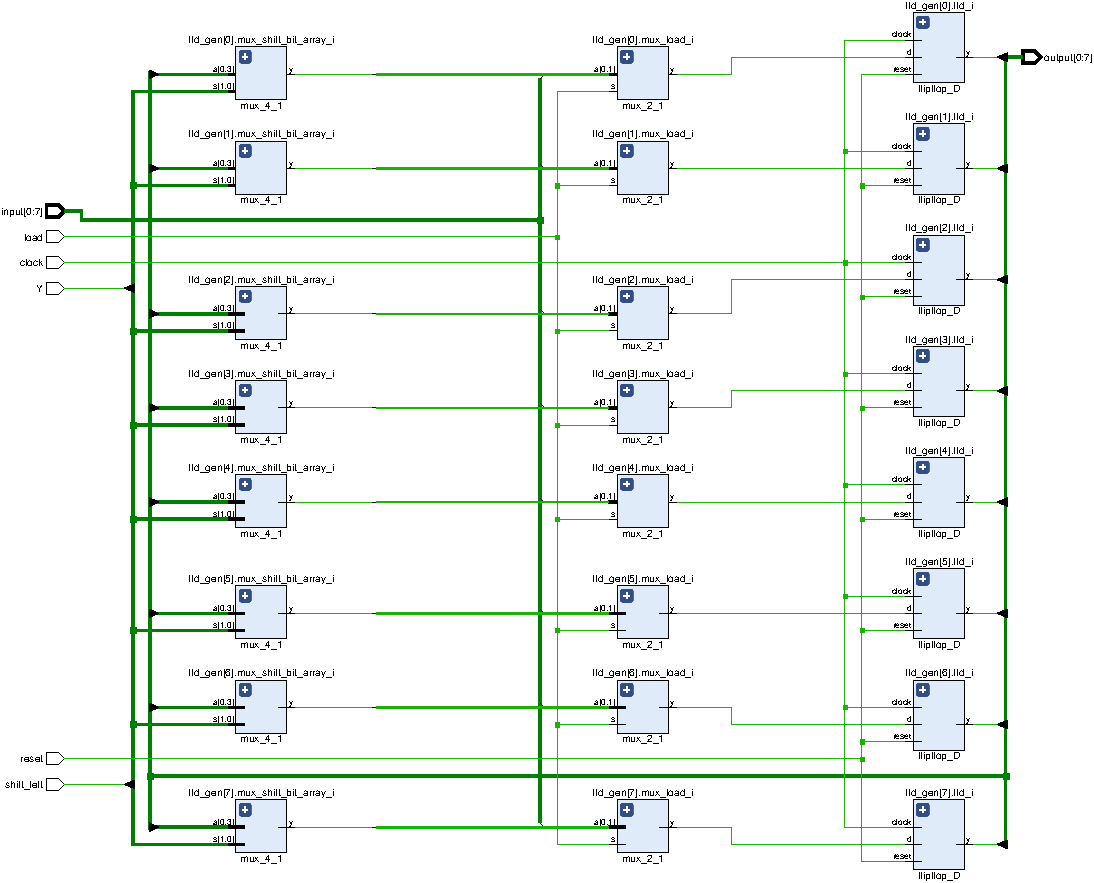
\includegraphics[width=\textwidth]{img/4_1_SHIFTREGISTER_STRUCTURAL.pdf}
    \caption{Schema a blocchi dello shift register strutturale con 8 bit}
    \label{fig:4_1_SHIFTREGISTER_STRUCTURAL}
\end{figure}

\subsubsection{Simulazione}

Per effettuare la simulazione il primo passo da compiere è la stesura del testbench. Prima di discutere quanto fatto è bene osservare il codice in figura:

\begin{code}
    \inputminted{vhdl}{vhdl/shiftregister_tb.vhd}
    \caption{Testbench degli shift register}
    \label{cod:shiftregister_tb}
\end{code}

Il testbench è utilizzato per verificare il corretto funzionamento di entrambe le versioni del registro a scorrimento:

\begin{enumerate}
    \item \texttt{shiftregister\_structural}: implementazione strutturale.
    \item \texttt{shiftregister\_behavioral}: implementazione comportamentale.
\end{enumerate}

La prima operazione svolta è stata la dichiarazione di un’entity. Si può notare che il corpo dell’entity è vuoto, poiché il testbench non rappresenta un componente hardware da implementare, ma serve esclusivamente per la simulazione e la verifica del corretto funzionamento del sistema.

L'architettura \texttt{behavioral} definisce:

\begin{itemize}
    \item I componenti \texttt{shiftregister\_structural} e \texttt{shiftregister\_behavioral} da testare.
    \item Costanti per la simulazione (\texttt{CLK\_period} per il clock e \texttt{bit\_number} per la dimensione del registro).
    \item Segnali per controllare i componenti (\texttt{clock}, \texttt{reset}, \texttt{load}, \texttt{input}, selezione \texttt{Y}, direzione \texttt{shift\_left}, e \texttt{output} attesi).
\end{itemize}

Vengono creati due Unit Under Test (\texttt{uut}):

\begin{itemize}
    \item \texttt{uut\_structural}: istanza della versione strutturale.
    \item \texttt{uut\_behavioral}: istanza della versione comportamentale.
\end{itemize}

Entrambi ricevono gli stessi segnali di controllo per confrontarne il comportamento.

Il processo \texttt{stim\_process} fornisce stimoli ai registri per verificarne il comportamento. Le fasi del test sono:

\begin{enumerate}
    \item Attesa iniziale di \texttt{100 ns} per stabilizzare il sistema.
    \item Caricamento del valore \texttt{6F5D} nel registro:
    \begin{itemize}
        \item \texttt{reset} viene disattivato (\texttt{reset = `0'}).
        \item \texttt{load} viene attivato (\texttt{load = `1'} per \texttt{10 ns}), poi riportato a \texttt{`0'}.
    \end{itemize}
    \item Verifica degli shift con \texttt{assert}:
    \begin{itemize}
        \item Caso \texttt{Y = `0'}, \texttt{shift\_left = `0'} (shift a destra di 1 posizione). Output atteso: \texttt{B7AE}.
        \item Caso \texttt{Y = `0'}, \texttt{shift\_left = `1'} (shift a sinistra di 1 posizione). Output atteso: \texttt{6F5D}.
        \item Caso \texttt{Y = `1'}, \texttt{shift\_left = `1'} (shift a sinistra di 2 posizioni). Output atteso: \texttt{BD75}.
        \item Caso \texttt{Y = `1'}, \texttt{shift\_left = `0'} (shift a destra di 2 posizioni). Output atteso: \texttt{6F5D}.
    \end{itemize}
\end{enumerate}

Se gli output attesi non corrispondono a quelli ottenuti, viene generato un errore con assert, ossia se il valore non è corretto, la simulazione si interrompe con un messaggio di errore [Figura \ref{fig:shiftregister_tb}].

\begin{figure}[h]
    \centering
    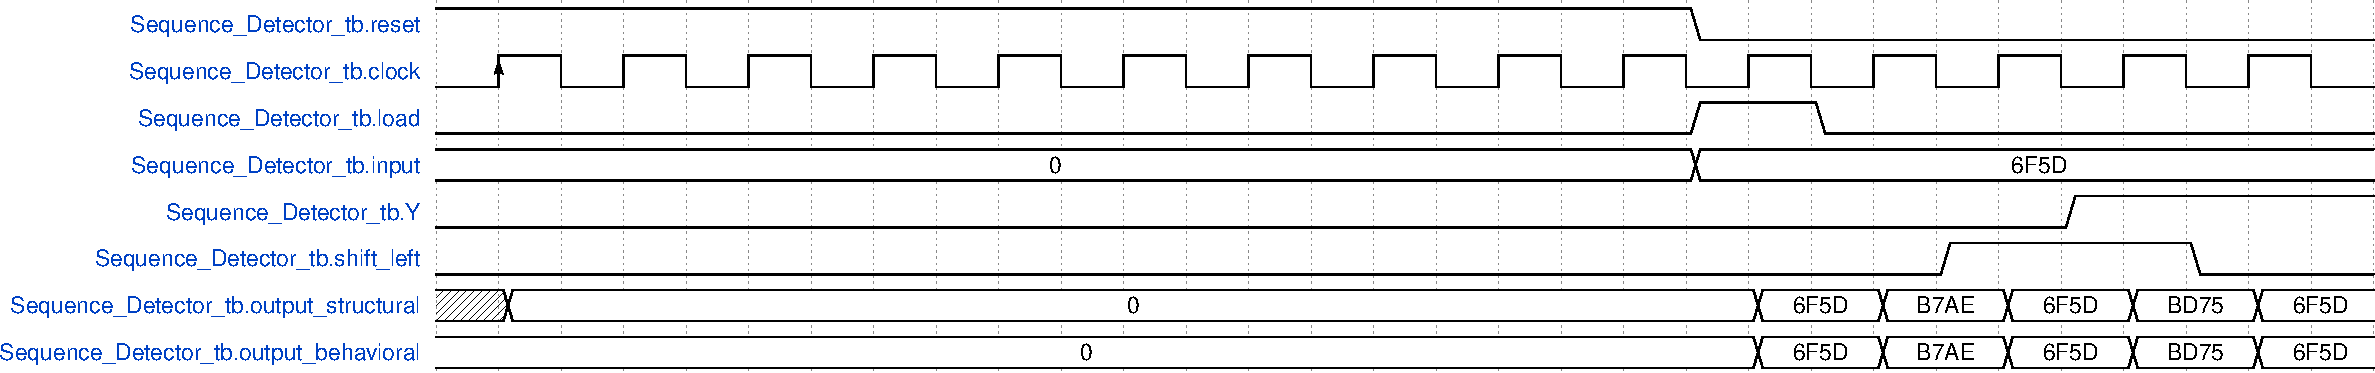
\includegraphics[width=\textwidth]{img/shiftregister_tb.pdf}
    \caption{Simulazione degli shift register}
    \label{fig:shiftregister_tb}
\end{figure}
